% Chapter 5 of Genesis
\bookchapter{The Family Of Adam}


\bverse This is the book of the genealogy\vmark{a} of Adam. In the day that God created man, He made him in the likeness of God.
	\contextnote{a}{Only the names of those leading to the genealogy of Noah are given. The others are not mentioned, but it is implied they exist in \bref{Genesis 5:4}, \bref{Genesis 5:7}, \bref{Genesis 5:10} and other scriptures.}

\bverse He created them male and female, and blessed them and called them Mankind in the day they were created.
\bverse And Adam\vmark{a} lived one hundred and thirty years, and begot \textit{a son} in his own likeness, after his image, and named him Seth.
	\translationnote{a}{The word/name `Adam' (Strong's 121\cite{Strong's GodRules}) means `red.' Other sources say this means `from red soil', `son of the red Earth', or similar translations.}

\bverse After he begot Seth, the days of Adam were eight hundred years; and he had sons and daughters.
\bverse So all the days that Adam lived were nine hundred and thirty years; and he died.
\bverse Seth\vmark{a} lived one hundred and five years, and begot Enosh.
	\translationnote{a}{The word/name `Seth' (Strong's 8352\cite{Strong's GodRules}) means `compensation.'}
	
\bverse After he begot Enosh, Seth lived eight hundred and seven years, and had sons and daughters.	
\bverse So all the days of Seth were nine hundred and twelve years; and he died.
\bverse Enosh\vmark{a} lived ninety years, and begot Cainan.
	\translationnote{a}{The word/name `Enosh' (Strong's 583\cite{Strong's GodRules}) means `man.'}
	
\bverse After he begot Cainan, Enosh lived eight hundred and fifteen years, and had sons and daughters.	
\bverse So all the days of Enosh were nine hundred and five years; and he died.
\bverse Cainan\vmark{a} lived seventy years, and begot Mahalalel.
	\translationnote{a}{The word/name `Cainan' (Strong's 7018\cite{Strong's GodRules}) means `possession.'}
	
\bverse After he begot Mahalalel, Cainan lived eight hundred and forty years, and had sons and daughters.	
\bverse So all the days of Cainan were nine hundred and ten years; and he died.
\bverse Mahalalel\vmark{a} lived sixty-five years, and begot Jared. 
	\translationnote{a}{The word/name `Mahalalel' (Strong's 4111\cite{Strong's GodRules}) means `praise of God.'}
	
\bverse After he begot Jared, Mahalalel lived eight hundred and thirty years, and had sons and daughters. 
\bverse So all the days of Mahalalel were eight hundred and ninety-five years; and he died.
\bverse Jared\vmark{a} lived one hundred and sixty-two years, and begot Enoch.
	\translationnote{a}{The word/name `Jared' (Strong's 3382\cite{Strong's GodRules}) means `descent.'}
	
\bverse After he begot Enoch, Jared lived eight hundred years and had sons and daughters.
\bverse So all the days of Jared were nine hundred and sixty-two years; and he died.
\bverse Enoch\vmark{a} lived sixty-five years, and begot Methuselah.
	\translationnote{a}{The word/name `Enoch' (Strong's 2585\cite{Strong's GodRules}) means `dedicated.'}
	
\bverse After he begot Methuselah, Enoch walked with God three hundred years, and had sons and daughters.
\bverse Soo all the days of Enoch were three hundred and sixty-five years.
\bverse And Enoch walked with God; and he \was not, for God took him.
	\questionnote{}{This scripture breaks the pattern seen with all the other members of this genealogy. With the others, their total days are numbered and they eventually die. However, with Enoch, it simply says `God took him' \textit{instead} of `he died.' What does this mean? Does this mean that God took him to another place, or that God took him in death early? Perhaps this can be a distinction between dying of old age (like the others) and dying of unnatural causes (in this case).}

\bverse 
\bverse 
\bverse 
\bverse 
\bverse 
\bverse 
\bverse 
\bverse 




\begin{figure}[htbp] % h=here, t=top, b=bottom, p=page
  \centering
  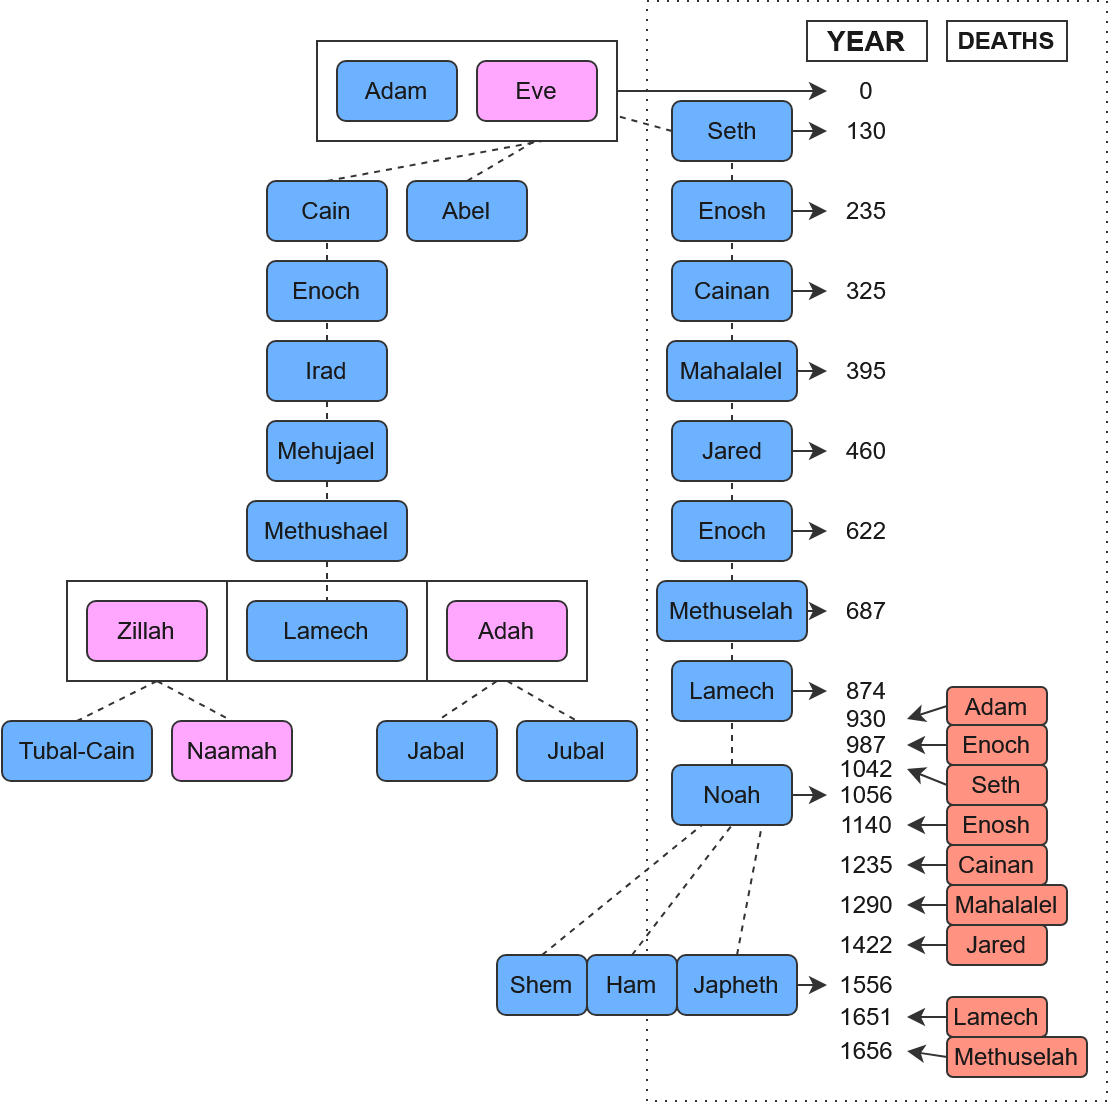
\includegraphics[width=\linewidth]{images/genealogies/noahs_genealogy.png}
  \caption{This is a diagram showing the genealogy of the family of Adam's as outlined in \bref{Genesis 4} and \bref{Genesis 5}. It ends with Noah's three children. Males are depicted in blue, while females are pink. Births are depicted as branching off from the mother. Marriages are depicted with a rectangular border around the couple. The genealogy between Seth and Noah have timeline markers showing the year of birth and death (death is shown for most, but not all). This diagram was created by me using the draw.io tool \cite{draw.io}.}
  \label{fig:noahs_genealogy}
\end{figure}